\documentclass[a4paper]{article}

%% Useful packages
\usepackage{amsmath}
\usepackage{graphicx}	
\usepackage{algpseudocode}
\usepackage{algorithm}
\usepackage[colorinlistoftodos]{todonotes}
\usepackage[colorlinks=true, allcolors=black]{hyperref}
\usepackage[fontsize=11pt]{scrextend}
\usepackage{titlesec}
 \usepackage[section]{placeins}

\setlength\parindent{0pt}
\titleformat*{\section}{\Large\bfseries}
\titleformat*{\subsection}{\Large\bfseries}

\title{PowerEnjoy Service - Design Document}

\begin{document}

\begin{titlepage}
\begin{figure}
\centering

\includegraphics[width=0.2\textwidth]{polimi.jpg}
\par
\LARGE Politecnico di Milano
\end{figure}


\maketitle
\textbf{Version 1.1}
\newline

\raggedright
Authors:
\begin{itemize}
	\item Domenico FAVARO (Mat. 837995)
        	\item Matheus FIM (Mat. 876069)
	\item Caio ZULIANI (Mat. 877266)	
\end{itemize}
\raggedleft
Prof. Elisabetta DI NITTO
\thispagestyle{empty}
\end{titlepage}

\tableofcontents
\newpage
 
\section{Introduction}
\subsection{Purpose}
This Design Document serves the purpose to present to all parties interested the description of the structure for the PowerEnjoy Service. It provides documentation of Software, Architecture and other important aspects of Design to help the understanding and development of the System. Every component that is implemented for the System will be explained as well as the purpose they serve to contribute to the fullfilment of all the project Requirements. All strategies and design decisions will be documented as well. Software Design Description, decisions and key information to be used to communicate the general purpose of the structure to our stakeholders, and serve as detailed documentation for the components of the System for the developers.

\subsection{Scope}
This Document presents the PowerEnjoy Service System, an electric car sharing service. To better understand the broader scope of the service, it is presented in the RASD Document. This Document will not include detailed information on all the tools and protocols that will be used in the development of the System but rather their purpose and functionality inside the PowerEnjoy System. As example, general knowledge of the Client-Server structure is expected as it will not be rigorously explained but instead how such structure will be used to satisfy our System's Requirements. 

\subsection{Glossary: Definitions, Acronyms, Abbreviations}
\begin{itemize}
\item \textbf{RASD:} Reqirements And Specifications Document.
\item \textbf{DD:} Design Document.
\item \textbf{Java EE:} Java Enterprise Edition. Software Development Platform.
\item \textbf{App:} Application. Refers to the deployed service as Web or Mobile Application.
\item \textbf{Component:} Software element that implements and offer functionalities in the System.
\item \textbf{EJB:} Enterprise Java Beans. Component in the Business Tier for the Application Logic.
\item \textbf{DBMS:} DataBase Management System.
\item \textbf{JDBC:} Java Database Connectivity, Java API to connect to DataBases.
\item \textbf{HTTPS:} Hypertext Transfer Protocol over TLS. Protocol to safefully communicate over the Internet.
\item \textbf{TLS:} Transport Layer Security that provides communication security.
\item \textbf{REST/RESTful:} Representational state transfer, architectural style for the System communications.
\item \textbf{MVC:} Model View Controller, software design pattern for implementing interfaces.
\item \textbf{API:} Application Programming Interface.
\end{itemize}
For other concepts concerning the Service definition look in the \textbf{Glossary} section of the RASD.

\subsection{Reference Documents}
\begin{itemize}
\item Specification Document: Assignments AA 2016-2017.pdf
\item PowerEnjoy Requirements And Specifications Document (RASD)
\item IEEE Std 1016-2009 IEEE Standard for Information Technology-Systems Designs-Software Design Descriptions (SDD IEEE 1016-2009.pdf)
\item Example Documents:
\begin{itemize}
\item[-] Sample Design Deliverable Discussed on Nov. 2.pdf
\item[-] Software Design Document (SDD) Template (sdd\_template.pdf)
\end{itemize}
\end{itemize}

\newpage
\subsection{Document Structure}
\begin{description}
\item \textbf{Section 1 - Introduction:} This section provides a general description of the purpose and structure of this Design Document.
\item \textbf{Section 2 - Architectural Design:} This section illustrates a broader to specific view of the components that form part of the System, presenting from the overview of the architecture of the system to a description of how each component will interface inside the structure.
\item \textbf{Section 3 - Algorithm Design:} Important functionalities of the System that require the development of algorithms will be described in this section.  
\item \textbf{Section 4 - User Interface Design:} All details refering to how the User will interface with the System, from the Web Application to the screens inside the Cars will be shown in this section. As well as general mockups of the Graphical User Interface (GUI) screens.
\item \textbf{Section 5 - Requirements Traceability:} In this section is explained how the Design decisions and structure help fulfill the Requirements for the System that were defined in the RASD. 
\item \textbf{Section 6 - Effort Spent:} Detailed record of the hours worked for each member of the team is documented in this section.
\item \textbf{Section 7 - References:} Any reference to additional external sources that can help the better understanding of this Document is documented in this section.
\end{description}

\newpage
\section{Architectural Design}
\subsection{Overview}
As was show in the Proposed System part of the RASD, the PowerEnjoy structure will consist on a 3-tier Client-Server Architecture. The server part built on a JEE Platform with access to the Company's Database Server and the Client consisting of Users, CRM and Cars that will use a browser to access our Web Application and a Mobile Device and Screen inside the Cars will access the Mobile Application.
As we need to interface our application with the Car functions (i.e. Lock, Unlock, Battery state) the application must have some Logic implemented client side. This distributed Logic structure will allow GUI to be created on the Client side as well.
The Database Server will belong to the Company and will allow registration of User, Reservations, Rides and Payments. Cars, CRM Employees and Parking Locations are asumed to be added outside of this System.

\begin{itemize}
\item Client Tier (Web App, Mobile App, Car)
\item Server Tier (Java EE Web and Application Server)
\item Enterprise Information System (EIS) Tier (DataBase Server)
\end{itemize}

\begin{figure}[h]
\centering
\vspace*{\fill}
\noindent\makebox[\textwidth]{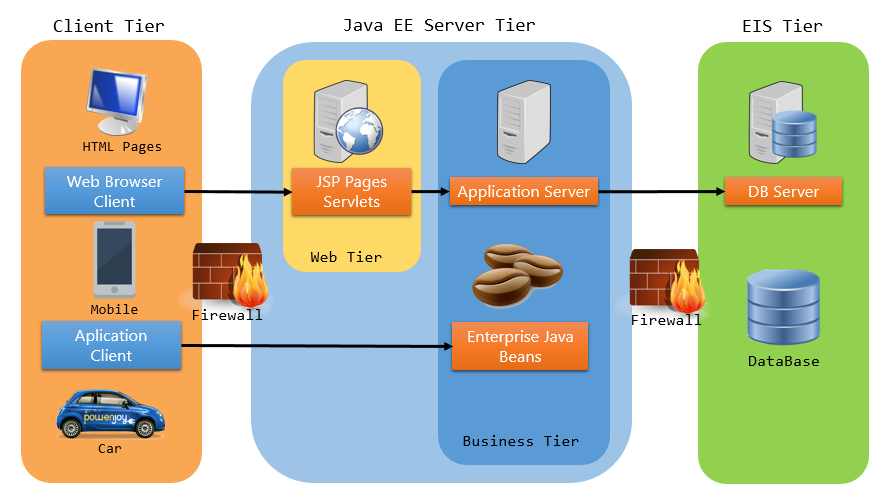
\includegraphics[width=1.2\textwidth]{ProposedSystemFW.png}}%
\caption {Proposed System Architecture}
\vspace*{0.5cm}
\end{figure}
\newpage

\subsection{High level components and their interaction}
Following our Architecture we organize the High level components on the 3 Tiers. This overview shows the interaction between the components and the entities they represent inside the System. Clients will have their User and CRM Components, distributed as Interfaces and Web Pages for the Apps. Inside the Server through Servlets and Session Beans a User and CRM Controllers will provide the services to the clients sending the requests with the respective Controllers. Based in the MVC pattern Controllers will manage the data that will be viewed by the Client. Each Controller will manage and represent the System Entities previously explained in the RASD and will interface with a Persistent DataBase Connection to the DBMS. Helpers and Extra Feature Components are represented as well.

\begin{figure}[h]
\centering
\vspace*{\fill}
\noindent\makebox[\textwidth]{\includegraphics[width=1.4\textwidth]{HighLevelComponents.png}}%
\caption {High Level Component Structure}
\vspace*{0.5cm}
\end{figure}

\newpage
\subsection{Component View}
\subsubsection{User Component}
Represents the User in the Client Tier that translates user actions and send requests to the UserController Component, then presents the output to the User. Is composed of several pages that present different types of information. Implement the Service Requests for each Actor, Web Pages in Web Server and Mobile Application and will have to interface with the central Server Component.
\subsubsection{CRM Component}
The CRM in the Client Tier will access just via browser, web server to the System. Is composed of a different set of pages that perform the requests to the CRM Controller.
\begin{figure}[h]
\centering
\vspace*{\fill}
\noindent\makebox[\textwidth]{\includegraphics[width=0.5\textwidth]{UserCRMComponents.png}}%
\caption {Client Components}
\vspace*{0.5cm}
\end{figure}
\subsubsection{Car Component}
Represents the Car outside of our system that presents an interface to provide information and receive commands from the Car Controller Component.
\subsubsection{Reservation Controller}
Manages the Reservations made by Users, when a reservation is corfirmed, it will create the correspondant Ride.
\subsubsection{Ride Controller}
Manages the Active Rides. When a ride is finished, it creates a Payment using the Payment Controller.
\subsubsection{Payment Controller}
Implements the Logic to make a Payment or Transaction to a User Account, using a PaymentHelper to interface with Credit Card and online Payment. Used by the Ride and the User Report Controllers.
\subsubsection{User Report Controller}
Used by the CRM Controller to generate User Reports.
\begin{figure}[h]
\centering
\vspace*{\fill}
\noindent\makebox[\textwidth]{\includegraphics[width=0.8\textwidth]{ReservationRidePaymentComponents.png}}%
\caption {Entity Controllers}
\vspace*{0.5cm}
\end{figure}
\subsubsection{User Controller}
Will handle the requests coming from the Users. Handle their Login, Registration and Session functionalities and redirect others to their respective controllers.
\subsubsection{CRM Controller}
Will handle the requests from CRMs. Similar to the UserController it will handle CRM Login and Session functionalities and redirect others to their respective controllers.
\newpage
\begin{figure}[h]
\centering
\vspace*{\fill}
\noindent\makebox[\textwidth]{\includegraphics[width=1.1\textwidth]{UserCRMControllers.png}}%
\caption {User CRM Controllers}
\vspace*{0.1cm}
\end{figure}
\subsubsection{Car Controller}
Will manage Cars Status, Locations and interface to Cars to send them instructions.
\begin{figure}[h]
\centering
\vspace*{\fill}
\noindent\makebox[\textwidth]{\includegraphics[width=0.7\textwidth]{CarControllerComponent.png}}%
\caption {Car Controller}
\vspace*{0.5cm}
\end{figure}
\subsubsection{Location Helper}
Will provide an interface for Location queries. Can interface to an external Service Provider API (Google Maps).
\subsubsection{Chat Service}
 Will provide the chat platform to provide a channel of communication between Users and available CRMs
\subsubsection{Email Helper}
Will allow the System to communicate via mail with the Users (password, payment).
\newpage
\subsubsection{DBMS} 
Each Controller will implement a Persistent Entity for each class that will be mapped on the DB.
The Structure of the DB will mirror the Classes in our System.
\begin{figure}[h]
\centering
\vspace*{\fill}
\noindent\makebox[\textwidth]{\includegraphics[width=0.6\textwidth]{DatabaseStructure.png}}%
\caption {Database Structure}
\vspace*{0.5cm}
\end{figure}

\newpage
\subsection{Deployment View}
A first proposal for the Deployment View shows our main components in their deployed hardware as seen in the proposed Architechture. Mainly our Web, Application and DB Servers and the Client Devices. Our proposal for the communication protocols include:
\begin{itemize} 
\item The Web Clients communicate to the Web Server via HTTPS. 
\item The Application Server exposes a RESTful API for the Web Server, Mobile Apps and Cars. 
\item The Application Server communicates with the DB Server using JDBC connection.
\end{itemize}
\begin{figure}[h]
\centering
\vspace*{\fill}
\noindent\makebox[\textwidth]{\includegraphics[width=1.2\textwidth]{DeploymentView.png}}%
\caption {Deployment View}
\vspace*{0.5cm}
\end{figure}
\newpage
\subsection{Runtime View}
\subsubsection{Runtime View Diagram for User's login}
\begin{figure}[h]
\centering
\vspace*{\fill}
\noindent\makebox[\textwidth]{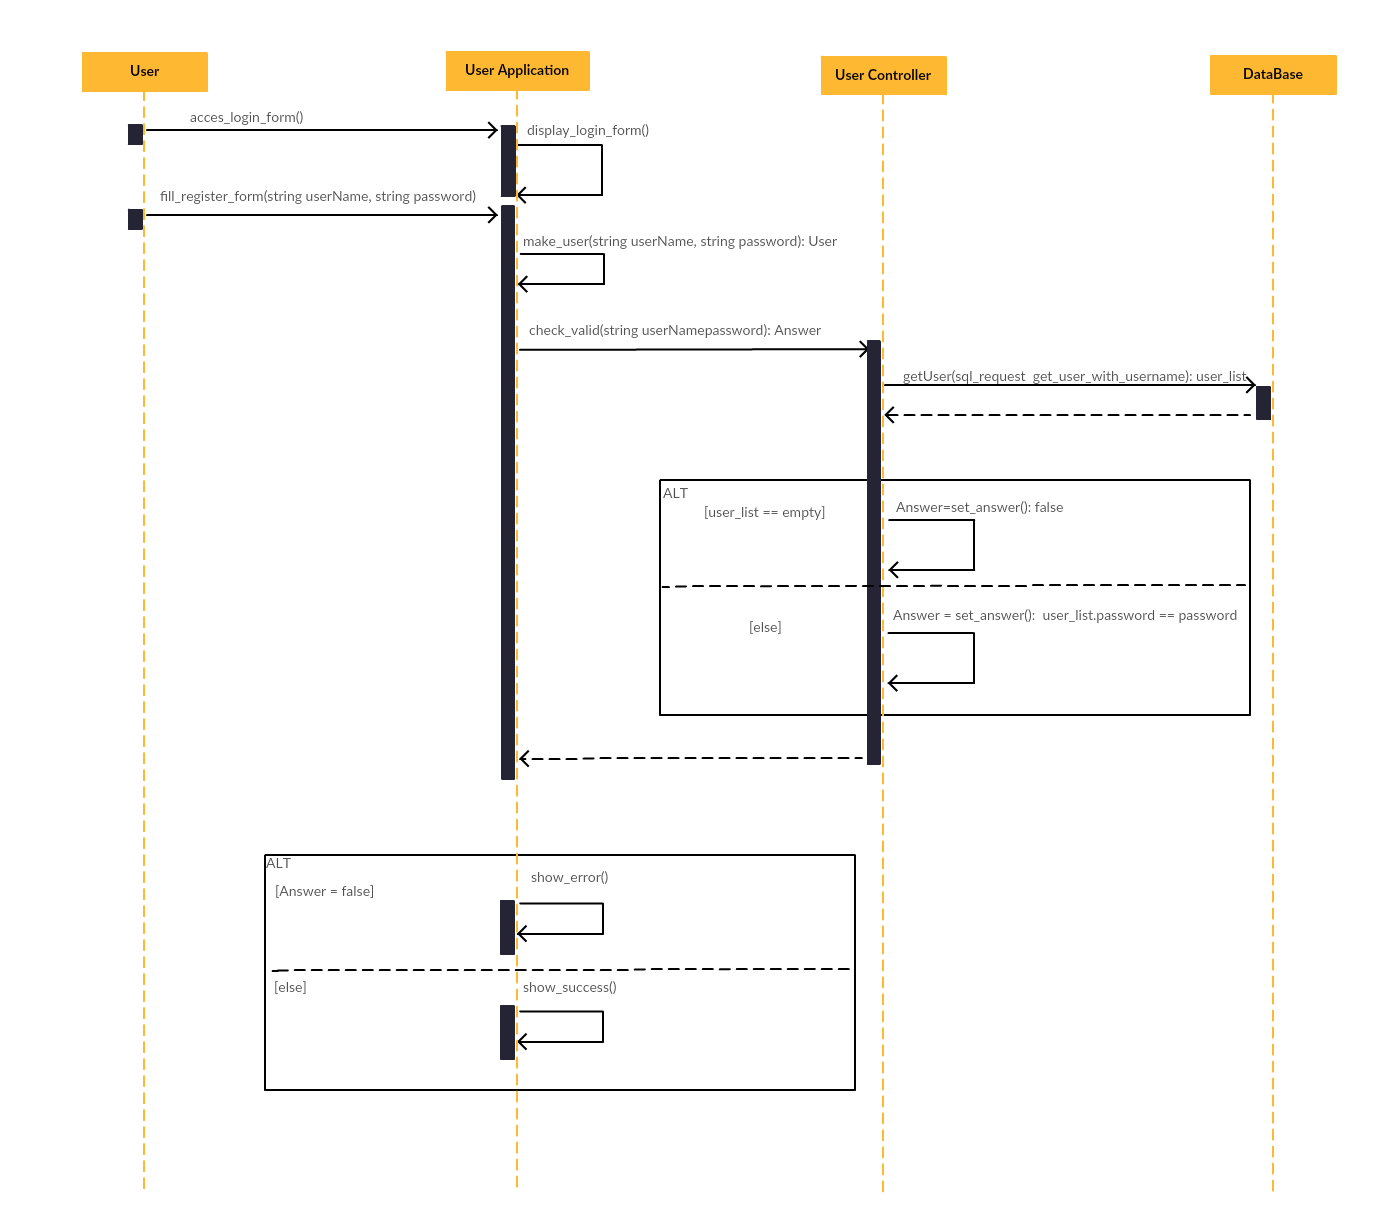
\includegraphics[width=1.5\textwidth]{RTuserLogin.png}}%
\vspace*{0.1cm}
\end{figure}
\newpage
\subsubsection{Runtime View Diagram for User's registration}
\begin{figure}[h]
\centering
\vspace*{\fill}
\noindent\makebox[\textwidth]{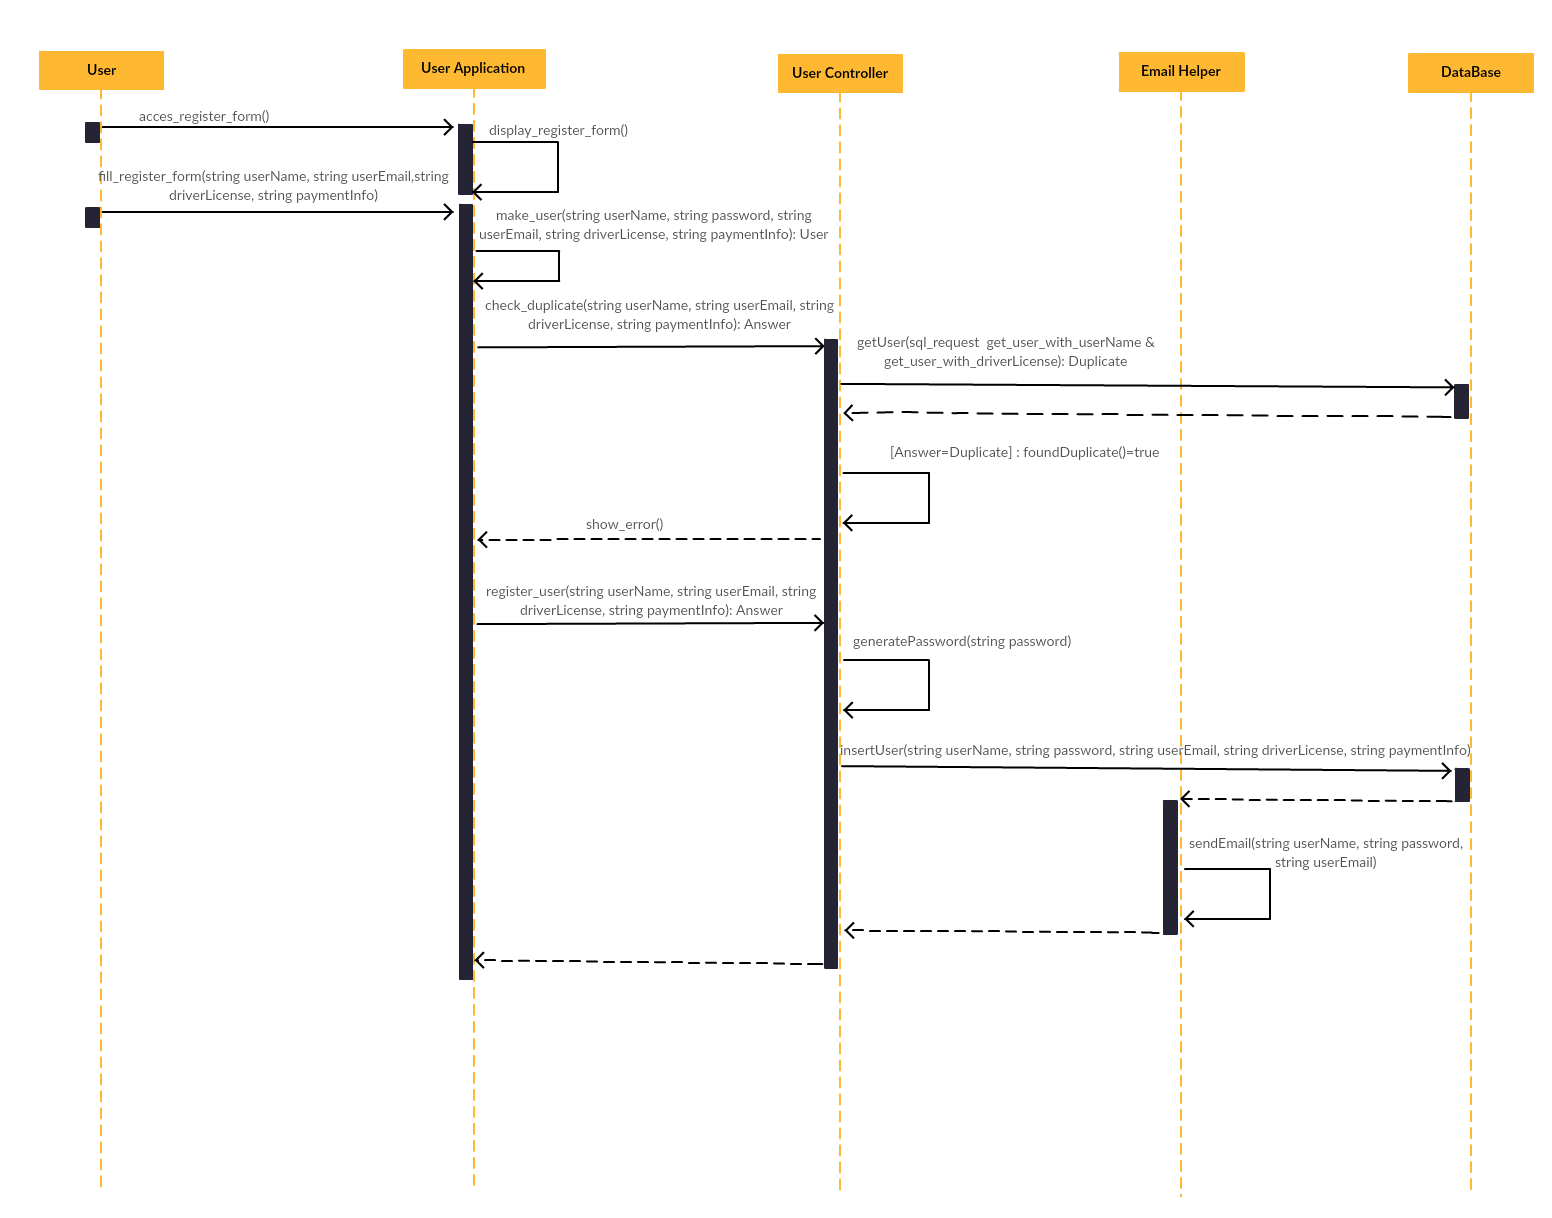
\includegraphics[width=1.5\textwidth]{RTRegisterUser.png}}%
\vspace*{0.1cm}
\end{figure}
\newpage
\subsubsection{Runtime View Diagram for the reserve of the car}
\begin{figure}[h]
\centering
\vspace*{\fill}
\noindent\makebox[\textwidth]{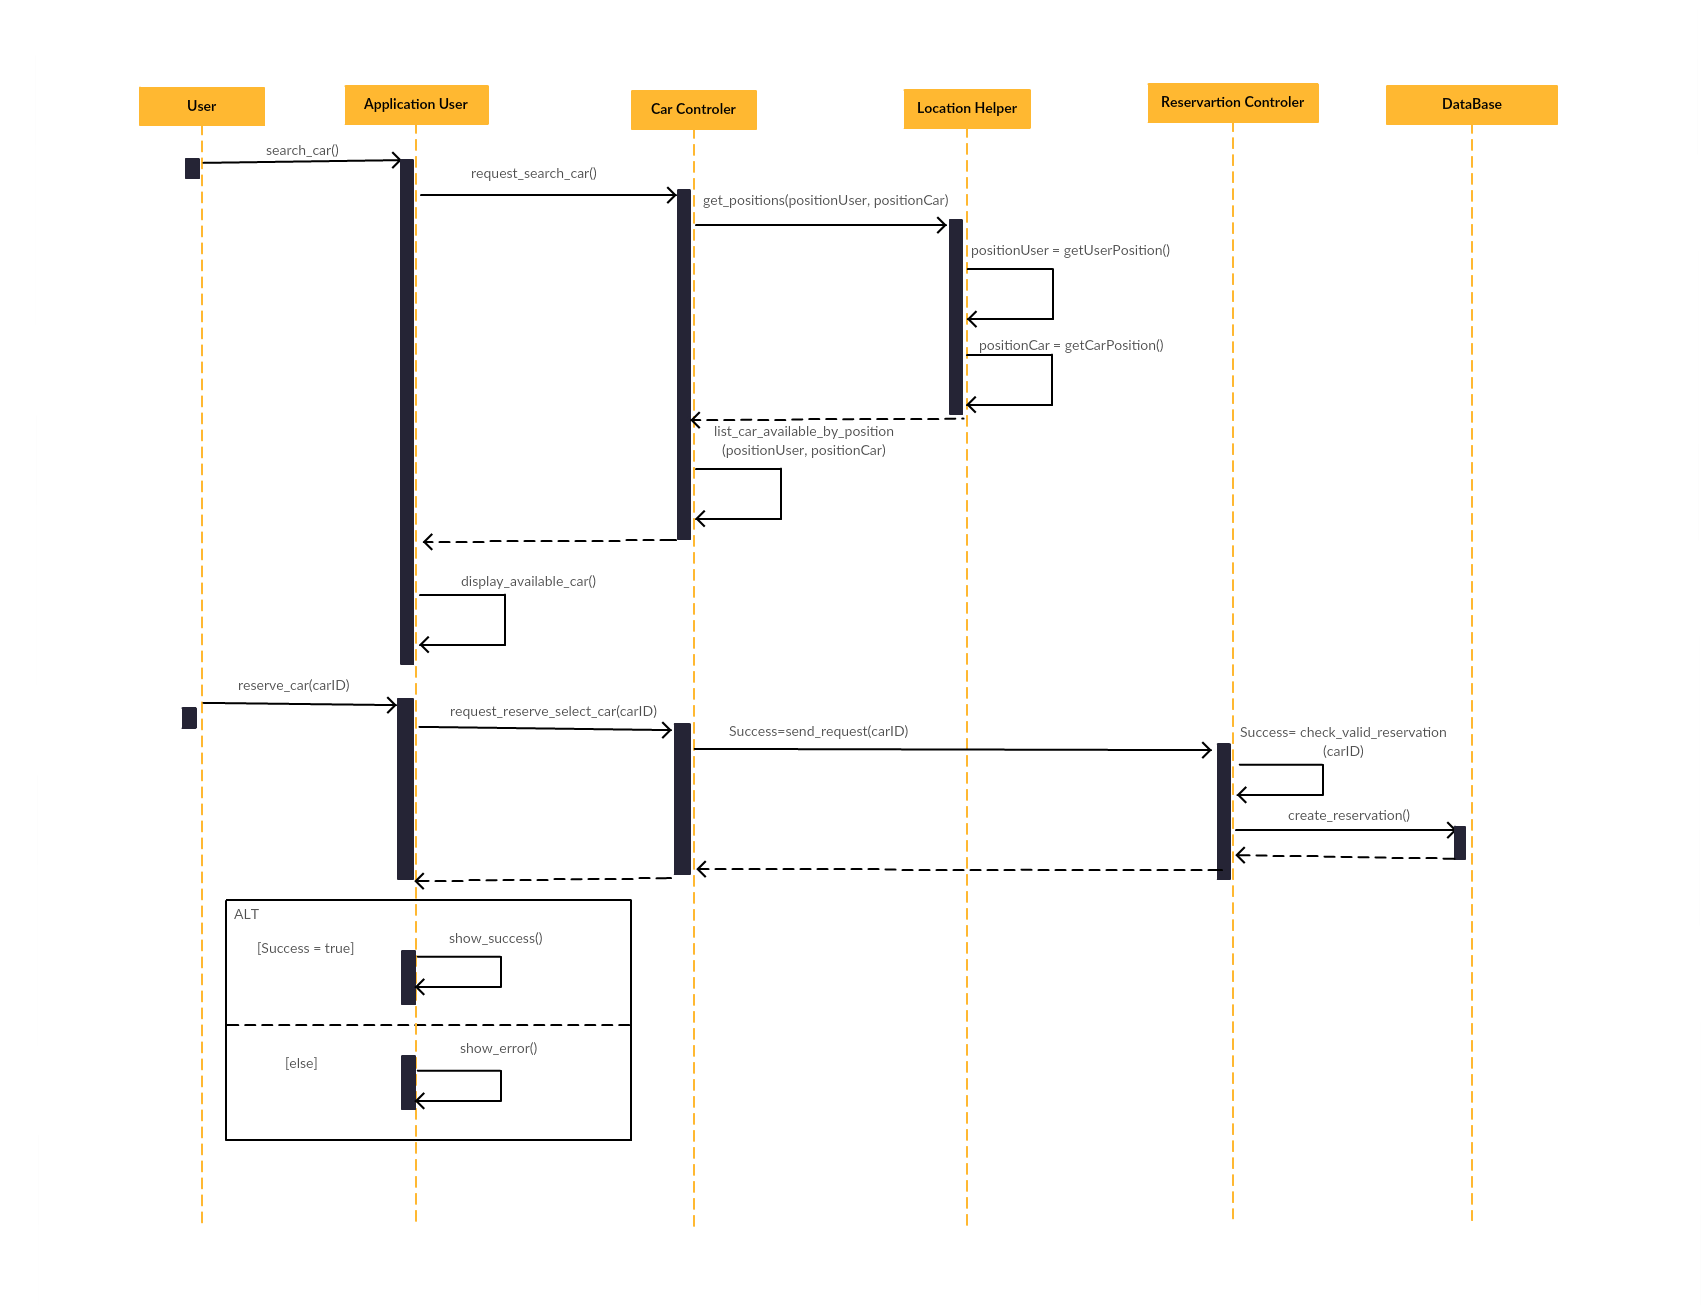
\includegraphics[width=1.5\textwidth]{RTreservation.png}}%
\vspace*{0.1cm}
\end{figure}
\newpage
\subsubsection{Runtime View Diagram for unlock the car}
\begin{figure}[h]
\centering
\vspace*{\fill}
\noindent\makebox[\textwidth]{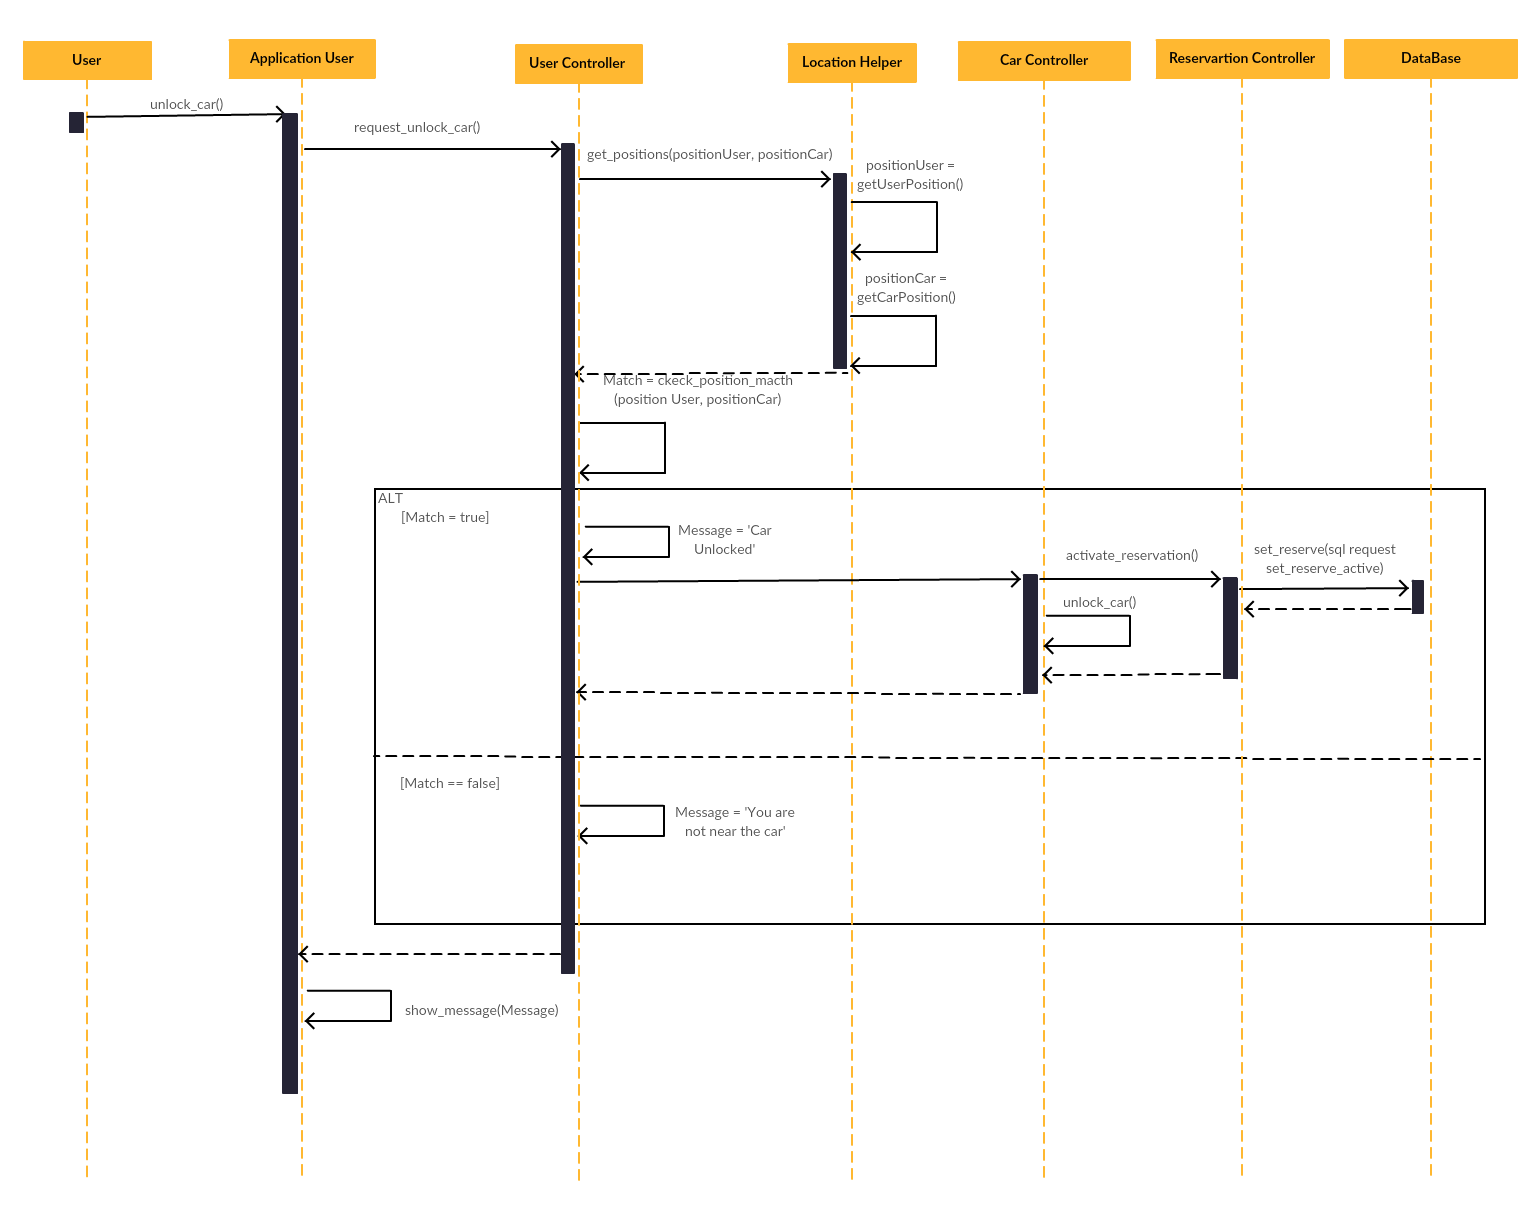
\includegraphics[width=1.5\textwidth]{RTunlockCar.png}}%
\vspace*{0.1cm}
\end{figure}
\newpage
\subsubsection{Runtime View Diagram where CRM create a Report of an User }
\begin{figure}[h]
\centering
\vspace*{\fill}
\noindent\makebox[\textwidth]{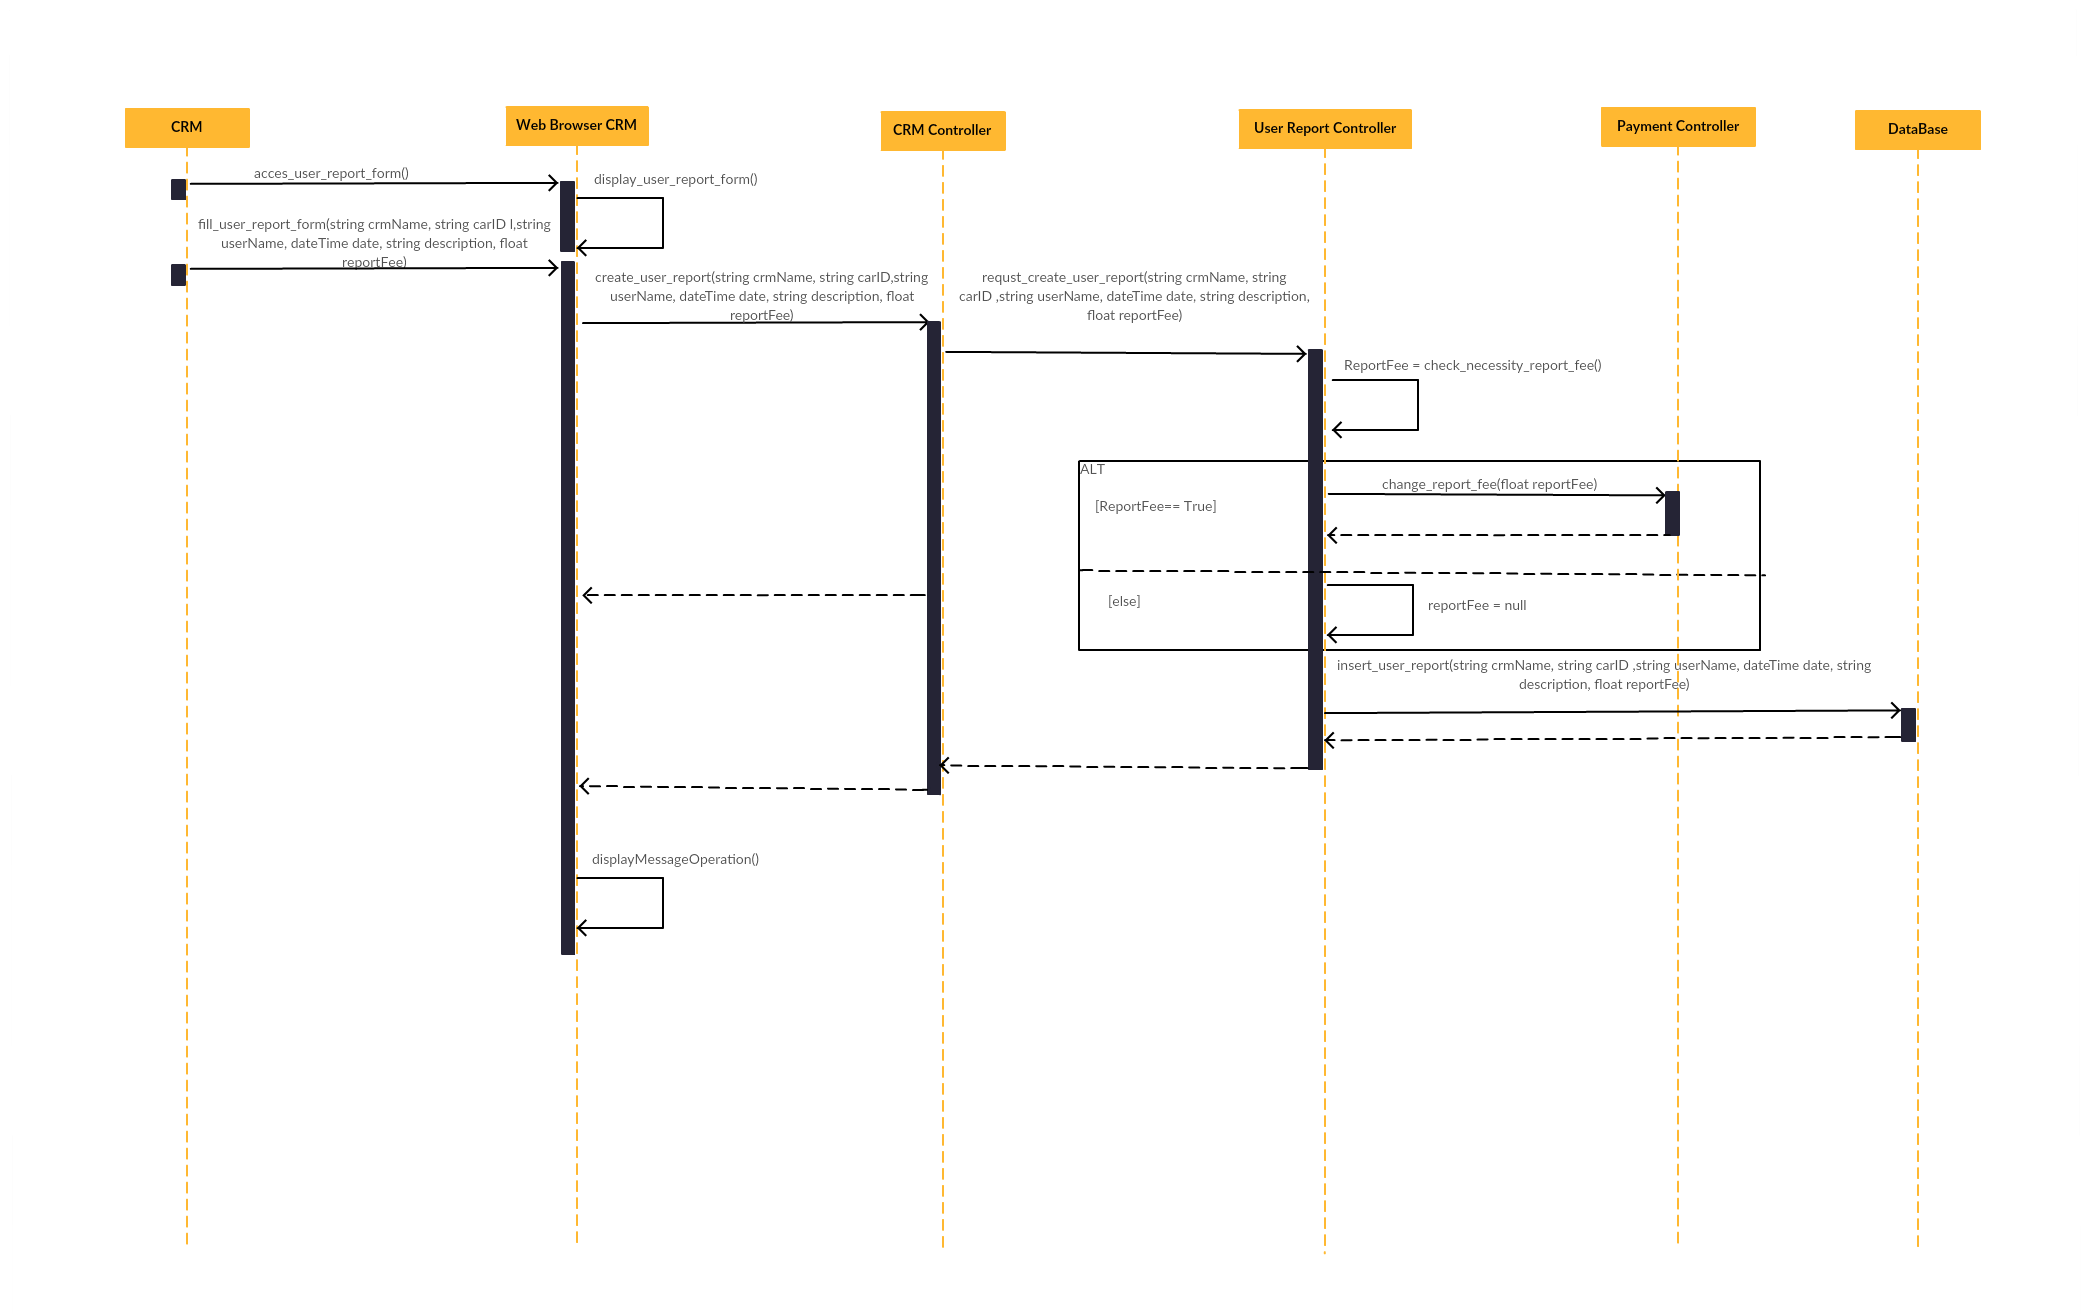
\includegraphics[width=1.5\textwidth]{RTcrmReport.png}}%
\vspace*{0.1cm}
\end{figure}

\newpage
\subsection{Component Interfaces}

\subsubsection{User Component}
\begin{figure}[h]
\centering
\vspace*{\fill}
\noindent\makebox[\textwidth]{\includegraphics[width=0.5\textwidth]{UserComponentInterface.png}}%
\vspace*{0.1cm}
\end{figure}

\subsubsection{Car Component}
\begin{figure}[h]
\centering
\vspace*{\fill}
\noindent\makebox[\textwidth]{\includegraphics[width=0.5\textwidth]{CarInterface.png}}%
\vspace*{0.1cm}
\end{figure}

\subsubsection{Reservation Controller}
\begin{figure}[h]
\centering
\vspace*{\fill}
\noindent\makebox[\textwidth]{\includegraphics[width=0.5\textwidth]{ReservationInterface.png}}%
\vspace*{0.1cm}
\end{figure}
\newpage

\subsubsection{Ride Controller}
\begin{figure}[h]
\centering
\vspace*{\fill}
\noindent\makebox[\textwidth]{\includegraphics[width=0.5\textwidth]{RideInterface.png}}%
\vspace*{0.1cm}
\end{figure}

\subsubsection{Payment Controller}
\begin{figure}[h]
\centering
\vspace*{\fill}
\noindent\makebox[\textwidth]{\includegraphics[width=0.5\textwidth]{PaymentInterface.png}}%
\vspace*{0.1cm}
\end{figure}

\subsubsection{User Report Controller}
\begin{figure}[h]
\centering
\vspace*{\fill}
\noindent\makebox[\textwidth]{\includegraphics[width=0.5\textwidth]{UserReportInterface.png}}%
\vspace*{0.1cm}
\end{figure}

\newpage
\subsubsection{User Controller}
Will Interface with the Users and answer requests redirecting them to the corresponding Controller.
\begin{figure}[h]
\centering
\vspace*{\fill}
\noindent\makebox[\textwidth]{\includegraphics[width=0.6\textwidth]{UserInterface.png}}%
\vspace*{0.1cm}
\end{figure}

\subsubsection{CRM Controller}
Will Interface with the CRM and answer their requests.
\begin{figure}[h]
\centering
\vspace*{\fill}
\noindent\makebox[\textwidth]{\includegraphics[width=0.6\textwidth]{CRMInterface.png}}%
\vspace*{0.1cm}
\end{figure}

\subsubsection{Car Controller}
The Car Controller will interface directly to the Car so as well to communicate the Car methods will offer these other methods.
\begin{figure}[h]
\centering
\vspace*{\fill}
\noindent\makebox[\textwidth]{\includegraphics[width=0.5\textwidth]{CarControllerInterface.png}}%
\vspace*{0.1cm}
\end{figure}

\subsubsection{Location Helper}
Location Helper will Implement our Location search Algorithms. It will help the System get the best ReCharging Station to ensure the best distribution of Cars in the city, as well as calculate Path and seach for nearby Cars or ReCharging Stations.
\begin{figure}[h]
\centering
\vspace*{\fill}
\noindent\makebox[\textwidth]{\includegraphics[width=0.7\textwidth]{LocationInterface.png}}%
\vspace*{0.1cm}
\end{figure}

\subsubsection{Chat Service}
\begin{figure}[h]
\centering
\vspace*{\fill}
\noindent\makebox[\textwidth]{\includegraphics[width=0.5\textwidth]{ChatInterface.png}}
\vspace*{0.1cm}
\end{figure}

\subsubsection{Email Helper}
\begin{figure}[h]
\centering
\vspace*{\fill}
\noindent\makebox[\textwidth]{\includegraphics[width=0.5\textwidth]{EmailInterface.png}}%
\vspace*{0.1cm}
\end{figure}

\subsection{Selected Architectural Styles and Patterns}
\subsubsection{MVC 3 Tier Architecture}
The 3 tier Architecture will be based in the MVC pattern as the Client represents the View, the Controllers will be implemented in the Application logic and the Model will be present in the Data Layer. This design allow us to present the data to our Users in a consistent and reliable way.
\subsubsection{Client-Server Architecture}
As the abstraction of our System is providing a service, the logical choice is to present the Client-Server model. The logic of our System implemented in our Servers and the Clients (Users and CRMs) will communicate with them to access our service. The simplicity and effectiveness of this model facilitates the deployment. Contrary to peer-to-peer 

\subsubsection{Communication: REST, HTTPS, JDBC}
\begin{itemize}
\item Basing our communication patterns on REST will allow simplicity for the Client requests, mantaining persistence on our data, this helps keeping the communication stateless. 
\item  REST over HTTPS is the most common practice and HTTPS is as well the standard secure protocol of communication on the Internet. 
\item Since we are deploying our App with Java EE, JDBC is the Java standard of communication with the DBMS.
\end{itemize}

\subsection{Other Design Decisions}
\begin{itemize} 
\item We decided to use Google Maps API for the Location Requests since it presents a familiar interface and its easy use and large support allows the manteinability of our service. We count on that Google Maps API will stay up to date for many years to come.
\end{itemize}


\newpage
\section{Algorithm Design}
\subsection{Making new Reservation}

Although this is not a complex algorithm, it is one of the main in the car sharing system. The goal in describing this is to rule out the other possibilities of implementation, in order to set the way smaller functions, that depend on the car reservation to operate, will handle their own tasks. The model that will be shown here has already been tested in the RASD file and was proved solid. \newline
Until the proper function is called the user will have to make a few steps:
\begin{itemize} 
\item From the home screen, the user will select a car near his position or near the address he/she entered.
\item  When a car is selected the user will see relevant information of the car, to help him decide whether or not make the reservation.
\item After the user has select the car and confirmed the reservation, the algorithm that will be displayed is called.
\end{itemize}
\begin{figure}[h]
\centering
\vspace*{\fill}
\noindent\makebox[\textwidth]{\includegraphics[width=0.5\textwidth]{CAR_RESERV.png}}%
\caption {Fluxogram for making a new reservation. "Cancel" steps were omitted but are possible every time.}
\vspace*{0.2cm}
\end{figure}

\begin{algorithm}
\caption{Making a new Reservation}\label{MakeReserv}
\begin{algorithmic}[1]
\Procedure{MakeReserv}{$Car, Account, ListOfReservations, listOfAvailableCars$}

\Comment{no user or car in two reservations }
\If{$Account \vee Car \subseteq ListOfReservations$}
	\State ShowErrorMessage
\Else
\State $Reservation \leftarrow CreateReserv(Car, Account)$ \Comment Sets the variables for the data structure
\State $ListOfReservations \leftarrow ListOfReservation + Reservation$
\State $listOfAvailableCars \leftarrow listOfAvailableCars - Car$
\State CounterTrigger($Reservation$) \Comment Starts Counter
\EndIf
\State \textbf{return} 
\EndProcedure
\end{algorithmic}
\end{algorithm}

The counter will work with interruptions. We have three main fases:
\begin{itemize} 
\item User picks up the car in time, counter is ended. 
\item 45 minutes has passed, notification is sent to the user.
\item 1 hour is reached and user is billed.
\end{itemize}

\begin{algorithm}[H]
\caption{Counter Trigger}\label{Counter}
\begin{algorithmic}[1]
\Procedure{Counter}{$Reservation$}

\Comment Different interruptions will trigger different parts of the function

\If {$45Min == TRUE$} \Comment time to issue a warning
	\State ShowWarning
	\State Wait \Comment system sleep
\EndIf


\If {$TimeFinished == TRUE$} \Comment 1 hour has passed
	\State ShowWarning
	\State $Ride \leftarrow createRide(Reservation)$
	\State $Ride.notPickUp \leftarrow 1$ 
	\State FeeCalc($Ride$) \Comment bill the user for not picking up
	\State \textbf{return}
\EndIf

\If {$PickUp == TRUE$} \Comment User nearby the car
	\State $StartRide(Reservation)$ \Comment unlock the car, take off reservation list and put on rides list
	\State \textbf{return}
\EndIf
 
\State Wait \Comment system is put to sleep
\EndProcedure
\end{algorithmic}
\end{algorithm}

\subsection{Calculating the fee}
This algorithm will be called when the car controller pass the signal that the engine is off, the car is parked in a safe area and the user is outside the car. \newline
The amount to be paid is calculated primarily based on the time of usage of the car and then extended for the virtuous behavior rules that add or subtract a percentage of the total amount. 
 These rules are:
\begin{itemize} 
\item  if the system detects the user took at least two other passengers for more than 50\% of the trip a discount of 10\% will be applied.
\item if the car is left with no more than 50\% of the battery empty, the system applies a discount of 20\%.
\item if the car is left more than 3km from the nearest power grid or with more than 80\% of the battery empty, the system charges 30\% more.
\item if a car is left at special parking areas and the user takes care of plugging the car into the power grid, the system applies 30\% discount.
\end{itemize}
If the user parks in a special parking area, where he can plug the car into a power grid, the closing of the invoice will be delayed in five minutes, in order to give time for the user to plug the car and receive the discount. 

\begin{algorithm}[H]
\caption{Part 1: Fee calculator}\label{Calc}
\begin{algorithmic}[1]
\Procedure{FeeCalc}{$Ride$}

\If {$Ride.notPickUp == TRUE$} 
	\State $Ride.Total \leftarrow 1$ \Comment 1 euro fee
	\State $Ride.Active \leftarrow FALSE$ \Comment Boolean
	\State $MarkCarAsActive(Ride.Car)$ \Comment car will be available again
	\State $PaymentHelper(Ride)$  \Comment Will charge the user
	\State $EmailHelper(Ride)$ \Comment Sent the invoice by e-mail 
\State
\Else
	\State $timeRide \leftarrow Ride.TimeOfDropOff - Ride.TimeOfPickUp$ \Comment Time is in minutes
	\State $timeFee \leftarrow timeRide * pricePerMin$
	\State
	\If {$Ride.PassengerDisc == TRUE$}
		\State $Disc \leftarrow Disc - 0.10$ \Comment Disc is initialized as 1
	\EndIf
	\State
	\If {$Ride.BatteryDisc == TRUE$}
		\State $Disc \leftarrow Disc - 0.20$
	\EndIf
	\State
	\If{$Ride.RecharginStationDisc == TRUE$}
		\State $Start5MinCounter()$ \Comment the user will be given 5 minutes to plug the car
		\If{$Ride.Car.plug == TRUE$}
			\State $Disc \leftarrow Disc - 0.30$
		\EndIf
	\EndIf
\algstore{break}
\end{algorithmic}
\end{algorithm}
This algorithm was divided in two parts:  In the first the "not picking up the car" condition is evaluated, the time fee is calculated and the discounts are added; In the second it is evaluated the bad usage of the car and the bills are charged.
\begin{algorithm}[H]
\caption{Part 2: Fee calculator}
\begin{algorithmic}[1]
\algrestore{break}
\State $EvaluateHarshConditions(Ride)$ \Comment Check if the car is more than 3 km of the nearest plug or it's with less then 20\% of battery 
	\State
	\If{$Ride.HarshConditionsFee == 1$}  \Comment User is charged extra for the trouble of recharging onspot 
		\State $Disc \leftarrow Disc + 0.30$ 
		\State $SignalizeCrm(Ride)$ \Comment Send message to crm crew that the car needs special attention
		\State $Total \leftarrow timeFee * Disc$  
		\State $PaymentHelper(Ride)$ 
		\State $EmailHelper(Ride)$ 
		\State \textbf{return}
	\EndIf
	\State
	\State $Ride.Total \leftarrow TimeFee * Disc$
	\State $PaymentHelper(Ride)$ 
	\State $EmailHelper(Ride)$
	\State $MarkCarAsActive(Ride.Car)$
	\State \textbf{return}
 \EndIf
\EndProcedure
\end{algorithmic}
\end{algorithm}

\subsection{Money-Saving}
When the money-saving option is enabled the system will suggest a power grid for the user to go in order to receive a discount. The algorithm for choosing the best place to send the user will take into account:
\begin{itemize} 
\item  The destination of the user, as no station within more than 1km will be suggested. In case there are no stations inside the 1 km radius, the system will apologize and show the nearest one. 
\item The suggestion will check if there are power plugs available in the location. In case they become unavailable after the start of the ride, the user will still receive the discount, as it is impossible to predict.
\item The algorithm will take in consideration the uniform distribution of the cars in the city.
\end{itemize}
The uniform distribution can be implemented in various different ways. As in the real world problem, it is impossible to have a uniform distribution (every point of the city with the same probability of having a car). But what can be done is to calculate the standard deviation for all the possible points and choose the destination that will increase it the most, as this means that the dispersion of the cars among the city are being broadened. And thus, staying a bit closer of the uniform distribution. \newline
As would be slow to calculate correctly the standard deviation every time, samples with a percentage of randomly chosen cars will be used instead.

\begin{algorithm}[H]
\caption{Money-Saving}\label{Money}
\begin{algorithmic}[1]
\Procedure{MoneySaving}{$Address, listOfAvailableCars$}

\State $Candidates \leftarrow PossiblePowerGrids(Address)$ \Comment will look for power grids within 1km of distance, returns a list

\If {$Candidates == EMPTY$} 
	\State $Suggest \leftarrow SearchPowerGrid(Address)$ \Comment return nearest Available power grid
	
	\State \textbf{return $Suggest$}

\Else 
	\State $Suggest \leftarrow StdDeviation(Candidates, listOfAvailableCars)$ \Comment calculate and return the best
\EndIf

\State \textbf{return $Suggest$}
\EndProcedure
\end{algorithmic}
\end{algorithm}

For the standard deviation, the correct formula would be: \\
\begin{math}
\sqrt[2]{\dfrac{\sum((x - \overline{x})^2 + (y - \overline{y})^2 )} {n-1}}
\end{math}  \\
But, as what is important for the decision is only the difference between the values, it's possible to notice in the following algorithm that the formula was simplified.


\begin{algorithm}[H]
\caption{Standard Deviation}\label{Std}
\begin{algorithmic}[1]
\Procedure{StdDeviation}{$Candidates, listOfAvailableCars$}
\Comment Candidates is a list of all possible locations
\State
\State $sampleSet \leftarrow ChooseCars(listOfAvailableCars)$ \Comment return a ramdom sample 2d-array with a fixed  number of locations.
\State
\For{$loc$  \textbf{in} $sampleSet$}
	\State$mean_x \leftarrow mean_x + loc.x$
	\State $mean_y \leftarrow mean_y + loc.y$
\EndFor
\State \Comment still needs to divide by the number of elements in the sampleSet
\State $mean_x \leftarrow mean_x \div |sampleSet|$ 
\State $mean_y \leftarrow mean_y \div |sampleSet|$
\State
\For{$Item$  \textbf{in} $ Candidates$}
	\State $sampleSet \leftarrow sampleSet + Item$
	\State
	\For {$loc$ \textbf{in} $sampleSet$}
		\State $deviation \leftarrow deviation + ((loc.x - mean_x)^2  + (loc.y - mean_y)^2)$ \Comment only the part that matters from the formula is used
	\EndFor
	\State
	\State $sampleSet \leftarrow sampleSet - Item$
	\State $deviation \leftarrow 0$
	\State
	\State \Comment savedDaviation starts with negative infinite
	\If {$deviation > savedDeviation $} 
		\State $ savedDeviation \leftarrow deviation$
		\State $Suggest \leftarrow Item$
	\EndIf		
\EndFor

\State \textbf{return $Suggest$}
\EndProcedure
\end{algorithmic}
\end{algorithm}



\newpage
\section{User Interface Design}
For our User Interface (UI) we'll offer a mobile App for Users and a desktop web App for Users and CRM. They will offer:

\begin {itemize}
\item \textbf{User experience diagram}
\begin{figure}[h]
\centering
\vspace*{\fill}
\noindent\makebox[\textwidth]{\includegraphics[width=1.3\textwidth]{uxUser.png}}%
\caption {User experience diagram for the User/Registered User.}
\vspace*{0.2cm}
\end{figure}
\newpage
\item \textbf{CRM experience diagram}
\begin{figure}[h]
\centering
\vspace*{\fill}
\noindent\makebox[\textwidth]{\includegraphics[width=1.2\textwidth]{uxCRM.png}}%
\caption {User experience diagram for the CRM.}
\vspace*{0.2cm}
\end{figure}
\pagebreak
\item MockUps for the MobileApp UI are presented in the RASD in section \textbf{4.2.1}. 
\item Following some WebApp UI examples not yet presented.
\begin{figure}[h]
\centering
\vspace*{\fill}
\noindent\makebox[\textwidth]{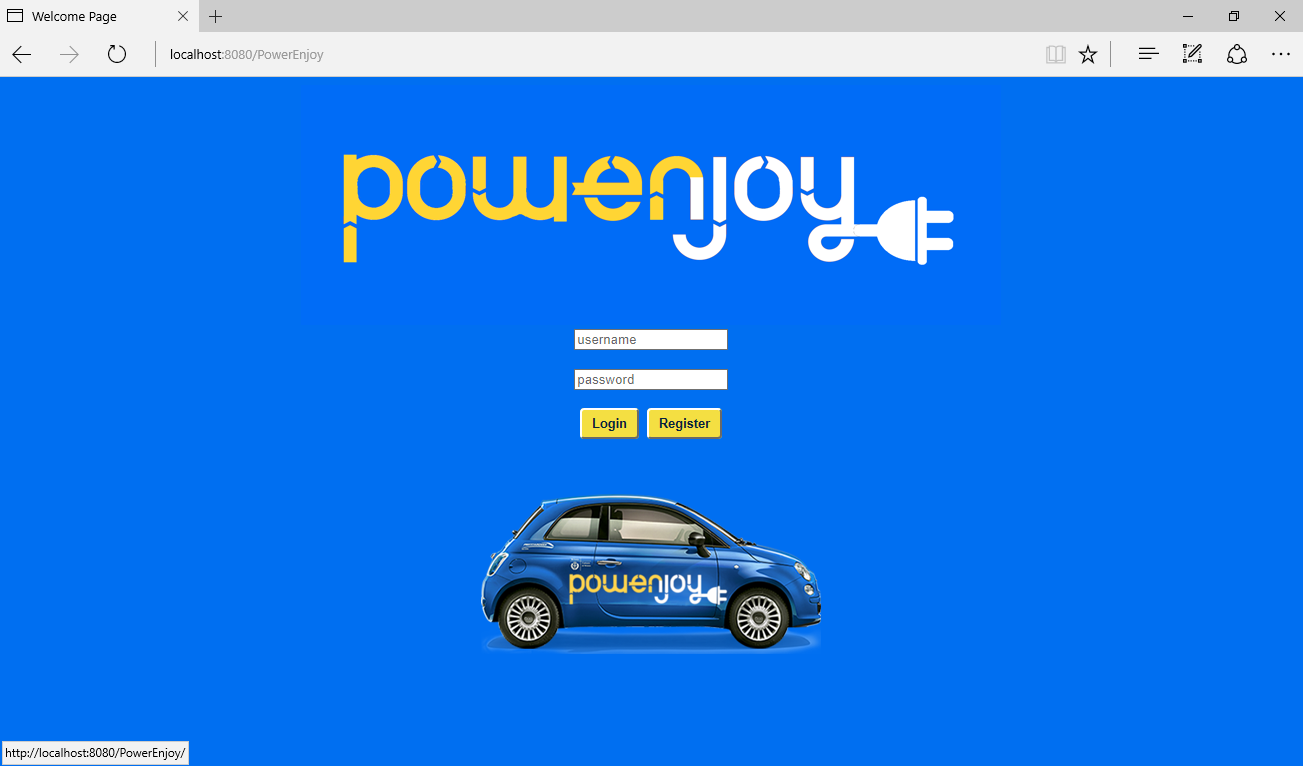
\includegraphics[width=0.8\textwidth]{BrowserLogInPage.png}}%
\caption {Browser LogIn Page}
\vspace*{0.2cm}
\end{figure}
\begin{figure}[h]
\centering
\vspace*{\fill}
\noindent\makebox[\textwidth]{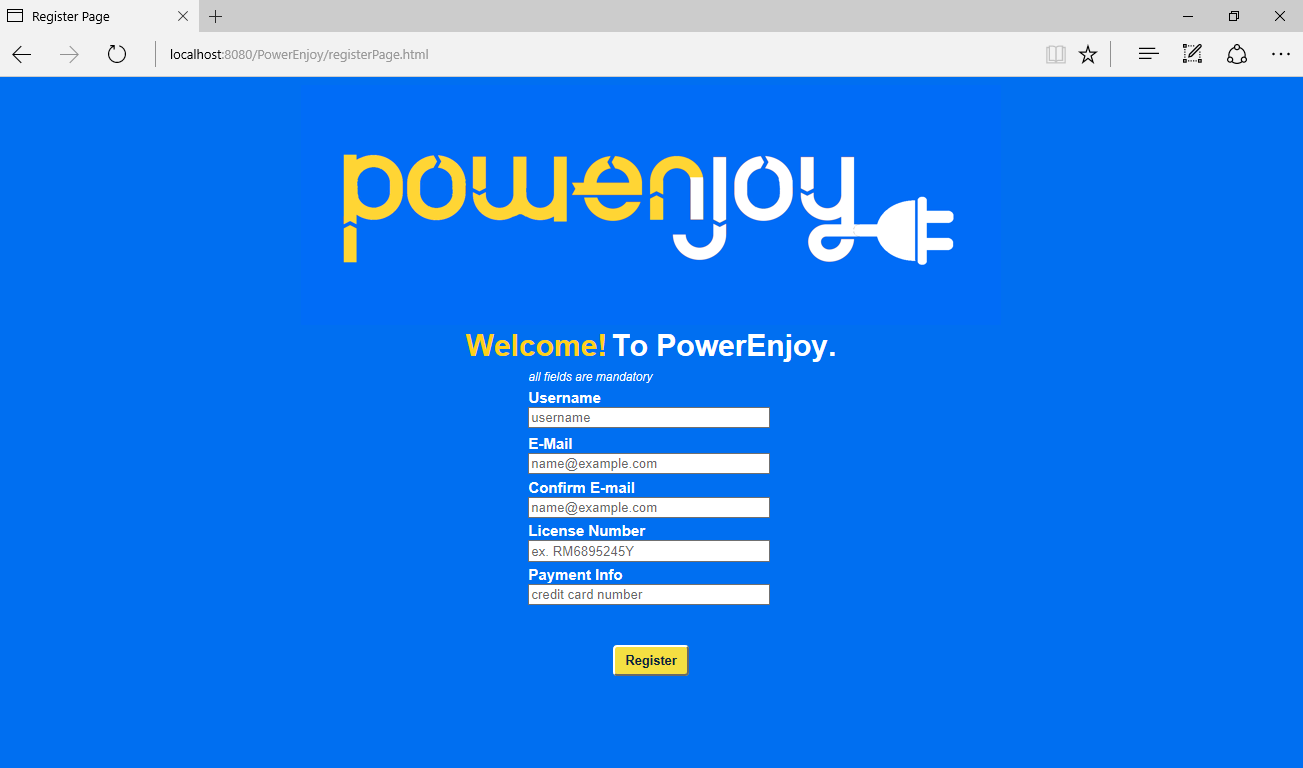
\includegraphics[width=0.8\textwidth]{BrowserRegisterPage.png}}%
\caption {Browser Register User Page}
\vspace*{0.2cm}
\end{figure}
\end{itemize}


\newpage
\section{Requirements Traceability}
\subsubsection{\textbf{User Requirements:}}
\begin{description}
\item [G.1)]First-Time Users must be able to register to the System creating an Account. 
\begin{itemize}
	\item[-]UserController will answer for the Registration Request andl add the User Account in the DB.
	\item[-]EmailHelper will send the Email with the Password to the User Email.
\end{itemize}
\item [G.2)]Registered Users must be able to login to their Account at any time they want.
\begin{itemize}
	\item[-]UserController will allow the Login Request checking the DB for the correct credentials.
\end{itemize}
\item [G.3)]Users can save his/hers credentials in the System.
\begin{itemize}
	\item[-]UserComponent in the Client side can be set to send the LogIn request automatically to the UserController whenever the App is opened.
\end{itemize}
\item [G.4)]A Registered User will be able to make a Reservation of any available Car near his/her current location or from an address that she/he can specify.
\begin{itemize}
	\item[-]UserController will answer the Search Car Request sending it to the CarController.
	\item[-]CarController will check all the available Cars and using the LocationHelper it will answer with the ones close to the User Location.
	\item[-]A Reservation Request will be forwarded to the ReservationController that will create it and add it to the DB.
\end{itemize}
\item [G.5)]Users that have made a Reservation must be able to notify the System when they are nearby the Reserved Car so the System can unlock it.
\begin{itemize}
	\item[-]UserController will control with the LocationHelper if the User and Car Location match.
	\item[-]ReservationController will be asked to activate the Reservation.
	\item[-]CarController will unlock the Car.	
\end{itemize}
\newpage
\item [G.6)]A User that has made a Reservation must be able to cancel it before 1 hour starting from the time when the Reservation was made.
\begin{itemize}
	\item[-]UserController will forward the Reservation Cancelation request to the ReservationController.
\end{itemize}
\item [G.7)]In case an User hasn't started using the Reserved Car at 45 minutes after the Reservation was made, he/she will be notified that either if the Reservation is not canceled or the Car is not used in 15 minutes, the Reservation will be automatically canceled and a 1 Euro fee will be charged to her/his Account.
\begin{itemize}
	\item[-]ReservationController will control for pending Reservations the start time. If it surpass the 45 minutes it will notify the EmailHelper to send the User a notification.
\end{itemize}
\item [G.8)]When Users start using their Reserved Car, they must be able to see their current expenses on the service through a System screen inside the Car.
\begin{itemize}
	\item[-]The CarComponent Screen will request the RideController the status of the Ride to show the expenses.
\end{itemize}
\item [G.9)]The User must be able to know where the safe parking areas are nearby his/her current location or any address that she/he can specify.
\begin{itemize}
	\item[-]UserController using the LocationHelper will request for Safe Parking Areas new the User.
\end{itemize}
\item [G.10)]Users must be able to finish their use of the Car when leaving it in a Safe Parking Area and exiting the car. The User will then be charged for the use of the service. The used Car will be locked and freed for Users to be reserved.
\begin{itemize}
	\item[-]The CarController is notified when the Car is stopped, ask the LocationHelper if it is in a Safe Parking Area.
	\item[-]If the Car sends the End Ride Request, the RideController will the end the Ride and ask the PaymentController to generate the Payment.
\end{itemize}
\item [G.11)]The User will always be notified when any Transaction is made on his Account.
\begin{itemize}
	\item[-]PaymentController when executes the transaction, asks the EmailHelper to send the User the Payment details.
\end{itemize}
\newpage
\item [G.12)]Notify the Users that are currently using a Car of any available discounts on their ride if they abide by the 'Virtuous Behaviour Rules' and of the extra fee in case of not respecting the facilitation of the re-charging of the Car on site. These extra discounts/charges will be applied on the Total fee at the end of the ride.
\begin{itemize}
	\item[-]The CarComponent will present this options to the User.
	\item[-]The RideController will calculate if any of them are applicable.
	\item[-]CarController will check for Car passengers, battery state and if it is plugged in.
	\item[-]LocationHelper will provide the Location for ReCharging Stations.
\end{itemize}

\item [G.13)]Users can activate the `Money Saving'a option on their Ride to be notified of any nearby Re-Charging station on their arrival destination. Leaving the car at the end of the ride at this station and plugging it will register as a 'Virtuous Behavior' and will apply and extra discount when charging the User.
\begin{itemize}
	\item[-]LocationHelper will search for the best ReCharging Stations considering a uniform distribution of parked cars and provide their Locations.
	\item[-]CarController Screen will show this ReCharging Stations nearby to the User's final destination.
\end{itemize}
\item [G.14)]Users must have the option to contact a CRM at any moment, the System must provide a Customer Service area that offers a Chat feature within the App or a phone number.
\begin{itemize}
	\item[-]ChatService will provide this feature.
\end{itemize}
\end{description}

\newpage
\subsubsection{\textbf{CRM Requirements:}}
\begin{description}
\item [G.15)]CRM must be able to log in into the System and see a list of all the Cars available, reserved, in use or unavailable.
\begin{itemize}
	\item[-]CRMController will send the LogIn Request to the CRM Controller to check correct credentials.
\end{itemize}
\item [G.16)]CRM has to be able to receive User Reports via chat or outside the app via phone call and be able to register it to the System.
\begin{itemize}
	\item[-]ChatService will find available CRM and contact it in cases of an User Request
\end{itemize}
\item [G.17)]CRM upon request form an User or any major cause can Reserve or cancel any active Reservation.
\begin{itemize}
	\item[-]ReservationController will provide different searchs for CRM Requests.
	\item[-]A Reservation Cancelation Request can be sent from a CRM to the ReservationController.
\end{itemize}
\item [G.18)]CRM must be able to change the Status of a Car given a User Report and tag it, in case it's unavailable, if it's due to Re-Charge, Fix, or Removal.
\begin{itemize}
	\item[-]CarController will offer this option to CRMs.
\end{itemize}
\item [G.19)]Upon the completion of an User Report CRM must be able to apply extra fees or refund the payment to any User in case the situation demands it.
\begin{itemize}
	\item[-]UserReportController will allow the Creation of a User Report in the DB.
	\item[-]If necessary the PaymentController will make a transaction linked with the User Report.
\end{itemize}
\end {description}

\newpage

\section{References}
\subsection{Used Tools}
Keeping track of the Tools used during develop the DD document were:
\begin{itemize}
	\item \textbf{GitHub:} for Version Control
	\item \textbf {Dia Diagram Editor:} for UML Diagrams
	\item \textbf {TeXworks:} for LaTex editing of this Document
\end{itemize}
\newpage
\subsection{Effort Spent}
\begin{tabular}{ | c | c | c | c | }
\hline
	\textbf {Date} & \textbf {Domenico} & \textbf {Caio} & \textbf {Matheus} \\ \hline
	27/11/16& 1h & 1h & 1h  \\ \hline
	28/11/16& 2h & - & - \\ \hline
	29/11/16& 2h & - & 2h\\ \hline
	30/11/16& 3h & - & 1h\\ \hline
	31/11/16& 1h & - & 2h\\ \hline
	01/12/16& - & 1h & - \\ \hline
	02/12/16& 5h & 2h & - \\ \hline
	03/12/16& 2h & 4h & - \\ \hline
	04/12/16& 2h & 4h & - \\ \hline
	05/12/16& 3h & - & - \\ \hline
	06/12/16& - & - & - \\ \hline
	07/12/16& - & - & 8h\\ \hline
	08/12/16& - & - & 6h\\ \hline
	09/12/16& - & 4h & - \\ \hline
	10/12/16& - & 2h & - \\ \hline
	11/12/16& 1h & 1h & 1h \\ \hline
\end{tabular}
\newpage

\section{Changelog}
As the project and design decisions may change during the development this document is also prone to change.
We'll document every version in this part.
\begin{itemize}
\item \textbf {Version 1.1:} 11/12/2016
\end{itemize}
\end{document}
